\levelB{Descriptive research on influence of number of classes}
\label{sec:numberofclasses}
\levelC{Objective}
In the previous section, it was observed that achieving 0.6 accuracy on file fragment classification using 30 classes was a difficult task to the considered models. In other studies results \cite{hiester_file_2018} \cite{sportiello_context-based_2012} \cite{amirani_feature-based_2013} \cite{maslim_distributed_2014} and on initial tests, the achieved accuracy for small number of classes was considerably higher. Hiester \cite{hiester_file_2018}, for instance, achieves 98\% accuracy using four classes.

This section investigates how the accuracy of the considered models change in relation to the number of classes in the dataset.


\levelC{Dataset}
Several independent models were trained with 2 to 30 \todo{change to 28 classes} extensions from the Govdocs1 dataset. For each number in the range 2 to 30, a random subset of extensions was selected to compose the dataset. Each extension has 200 file samples, half placed in the training dataset and half in the validation dataset. Each dataset was used to train a new model, that should distinguish between the selected subset of extensions in that filtered dataset. This process was repeated five times.



In addition to this sampling of extensions using different quantity of classes, all 435 combinations of pairs of extensions were compared. Each pair was used to compose a dataset and to train a new model for each one, using the same process described above.

\levelC{Models}
The same sampling, input, and output details described in section \ref{sec:evalmodels} were used here. The model that gave best results in that section, identified as ``CLD'', was selected to be used.

\levelC{Results}
% decrease in accuracy
Figure \ref{fig:nclasses} shows the graph of accuracy versus number of classes for the ``CLD'' model. The bottom line indicates, for comparison, what the accuracy would be for a random change classifier. An increase in number of classes appears to be  correlated with a decrease in accuracy. Another relevant aspect of the graph, is that the range of the results seems to be smaller when more classes are used.  

This pattern is understandable: as the number of classes grows, the harder the classification problem is, leading to a decrease in accuracy, while the individual contributions of each class to overall result diminishes, leading to an increase in precision.

This behavior is an important aspect to consider during the evaluation of file fragments studies. As Beebe et al. \cite{beebe_sceadan:_2013} have mentioned, studies that select fewer classes tends to yield higher results. 

Still, with 55\% of samples being misclassified when the number of classes is 30, the question of what are the error sources and how they can be addressed requires attention.

\noindent
\begin{figure*}[htb!]
\centering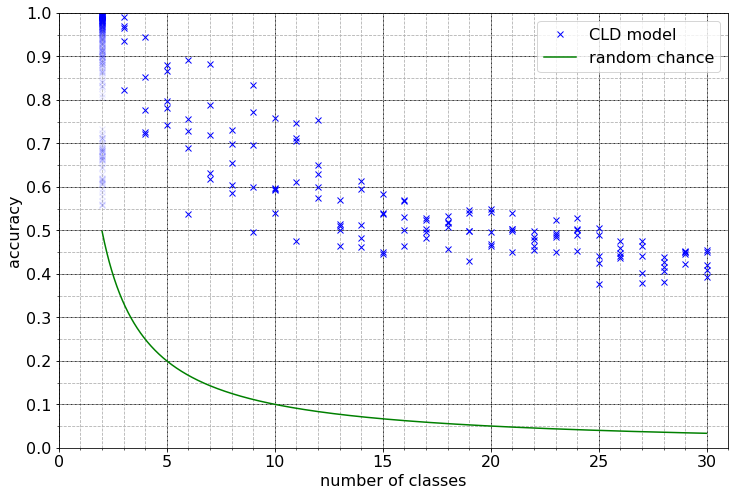
\includegraphics[width=1.0\textwidth]{content/nclasses.png}
\caption{\label{fig:nclasses}Validation accuracy by number of classes}%
\end{figure*}

\todo[inline]{graph was generated without text and unk classes}

Figure \ref{fig:dual} shows the graph of accuracy of each class when compared individually with each one of the others. Generally, file types with higher entropy tends to have lower minima, with the GIF file type being a notable exception. Most of these files use some form of compression, like image files for example. 


\noindent
\begin{figure*}[htb!]
\centering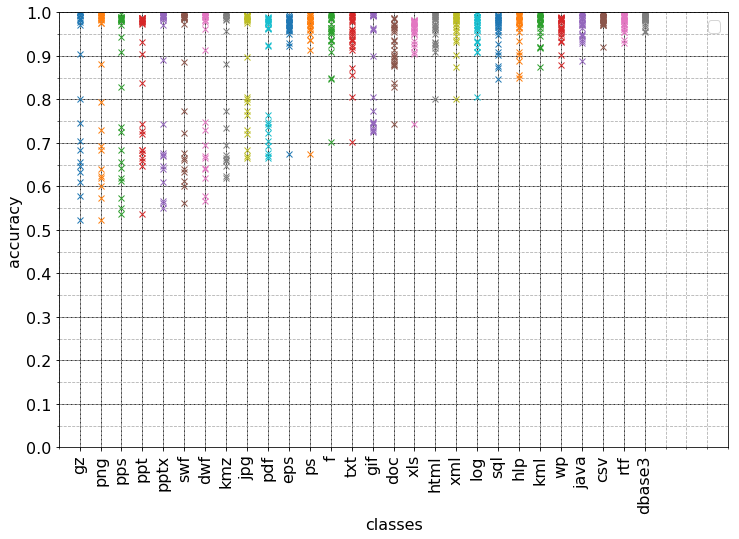
\includegraphics[width=1.0\textwidth]{content/dual.png}
\caption{\label{fig:dual}Validation accuracy of models trained with pair of classes}%
\end{figure*}


The accuracy obtained after the training of models with pair of classes was used to build a 28x28 matrix \todo{should rebuild with 30?}, using 0.5 in the main diagonal entries. This number was chosen because a pair of indistinguishable classes would have this accuracy in average. Then, a Principal Component Analysis (PCA) \todo{citation} was used to treat this matrix. The result is shown in figures \ref{fig:pca} and \ref{fig:pca2}. Again some file types with high entropy emerge as a promising group, ``dwf'',
``jpg'',
``pps'',
``ppt'',
``gz'',
``png'',
``pptx'',
``swf'',
``kmz'',
and ``pdf''.

\noindent
\begin{figure*}[htb!]
\centering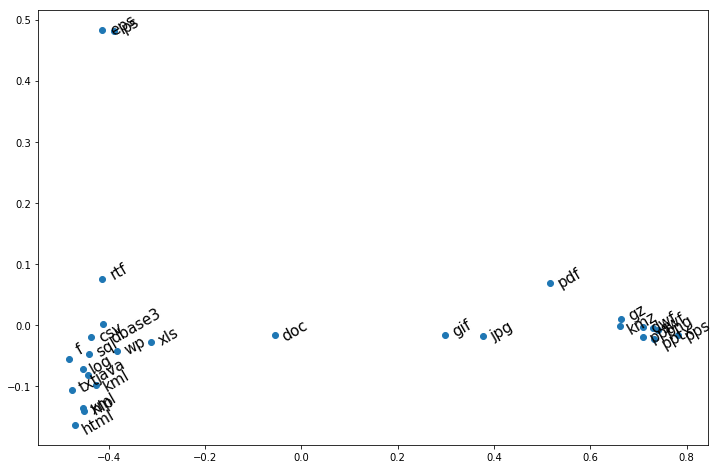
\includegraphics[width=1.0\textwidth]{content/pca.png}
\caption{\label{fig:pca}PCA of accuracy of models trained with pair of classes}%
\end{figure*}


\noindent
\begin{figure*}[htb!]
\centering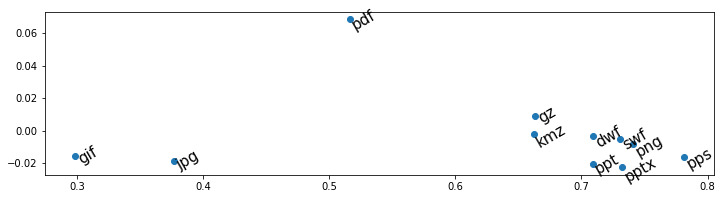
\includegraphics[width=1.0\textwidth]{content/pca2.png}
\caption{\label{fig:pca2}PCA of accuracy of models trained with pair of classes - detail}%
\end{figure*}


% the problem of unseen file types
% \levelC{Limitations and threats to validity}
